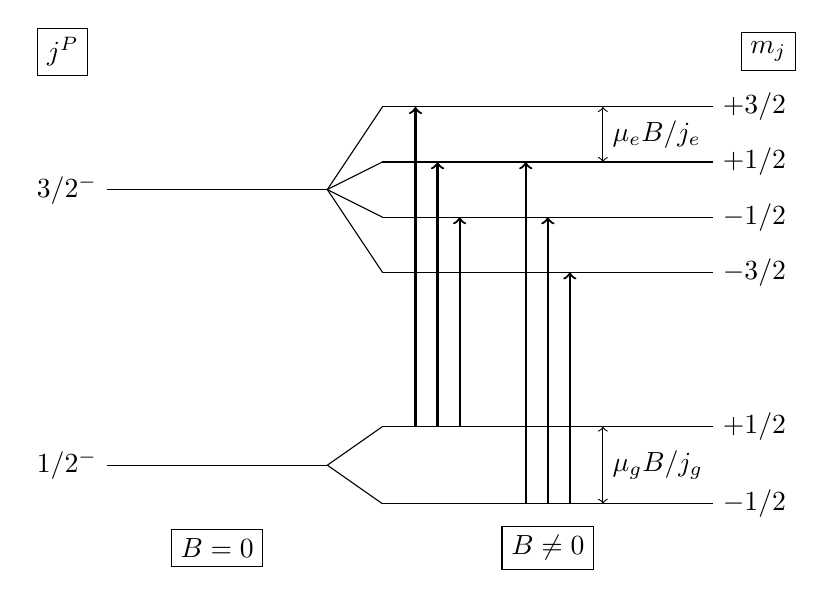
\begin{tikzpicture}[scale=1.4]
    \draw (0, 0) -- ++(3, 0) node[right] {$+3/2$};
    \draw (0, -0.5) -- ++(3, 0) node[right] {$+1/2$};
    \draw (0, -1) -- ++(3, 0) node[right] {$-1/2$};
    \draw (0, -1.5) -- ++(3, 0) node[right] {$-3/2$};

    \draw (0, -2.9) -- ++(3, 0) node[right] {$+1/2$};
    \draw (0, -3.6) -- ++(3, 0) node[right] {$-1/2$};

    \draw (-0.5, -0.75) -- (0, 0);
    \draw (-0.5, -0.75) -- (0, -.5);
    \draw (-0.5, -0.75) -- (0, -1);
    \draw (-0.5, -0.75) -- (0, -1.5);

    \draw (-0.5, -3.25) -- (0, -2.9);
    \draw (-0.5, -3.25) -- (0, -3.6);

    \draw (-0.5, -0.75) -- ++(-2, 0) node[left] {$3/2^-$};
    \draw (-0.5, -3.25) -- ++(-2, 0) node[left] {$1/2^-$};

    \draw[<-, thick] (0.3, 0) -- ++(0, -2.9);
    \draw[<-, thick] (0.5, -0.5) -- ++(0, -2.4);
    \draw[<-, thick] (0.7, -1) -- ++(0, -1.9);

    \draw[<-, thick] (1.3, -0.5) -- ++(0, -3.1);
    \draw[<-, thick] (1.5, -1) -- ++(0, -2.6);
    \draw[<-, thick] (1.7, -1.5) -- ++(0, -2.1);

    \draw[<->] (2, 0) -- ++(0, -0.5) node[midway, right] {$\mu_\text e B / j_\text e$};
    \draw[<->] (2, -2.9) -- ++(0, -0.7) node[midway, right] {$\mu_\text g B / j_\text g$};

    \node[draw] at (3.5, 0.5) {$m_j$};
    \node[draw] at (-2.9, 0.5) {$j^P$};

    \node[draw] at (-1.5, -4) {$B = 0$};
    \node[draw] at (1.5, -4) {$B \neq 0$};
\end{tikzpicture}
